\begin{frame}
\begin{itemize}
    \item What are Normalizing Flows
    \item NICE
    \item RealNVP
    \item \textbf{\color{red}{GLOW}}
    \item GamePlan
    \item Results
\end{itemize}
\end{frame}

\begin{frame}
    \frametitle{GLOW (Steven)}
    \begin{itemize}
        \item Builds from NICE and RealNVP.
        \item Uses 1x1 invertible convolutions which act as the permutation
            matrix from previous works.
        \item Gives high quality and sharp images.
    \end{itemize}
\end{frame}

\begin{frame}
    \frametitle{GLOW (Steven)}
    \center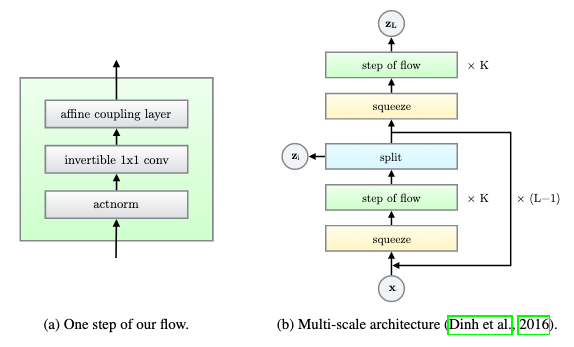
\includegraphics[width=0.75\textwidth]{GLOWFlow.png}\\
    \center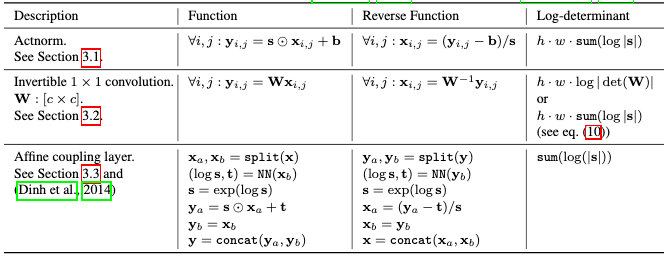
\includegraphics[width=0.75\textwidth]{GLOWComposition.png}
\end{frame}

\begin{frame}
    \frametitle{GLOW (Steven)}
    \center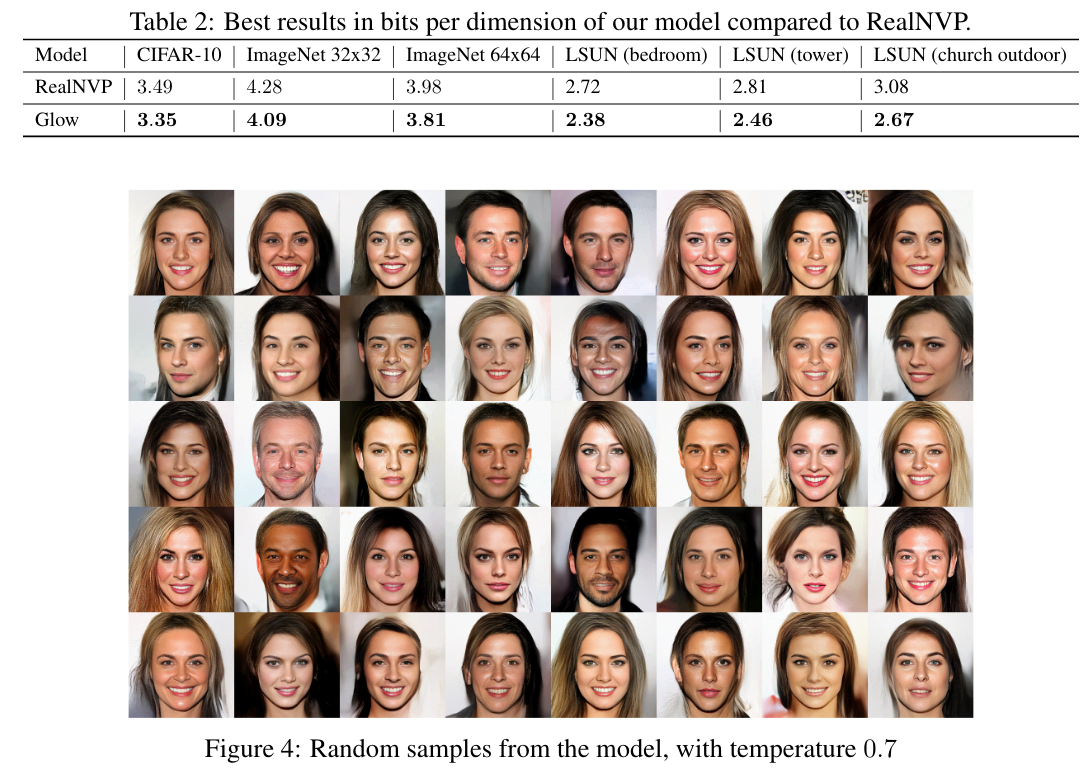
\includegraphics[width=0.75\textwidth]{GLOWResults.png}
\end{frame}

\begin{frame}
    \frametitle{GLOW (Steven)}
    \center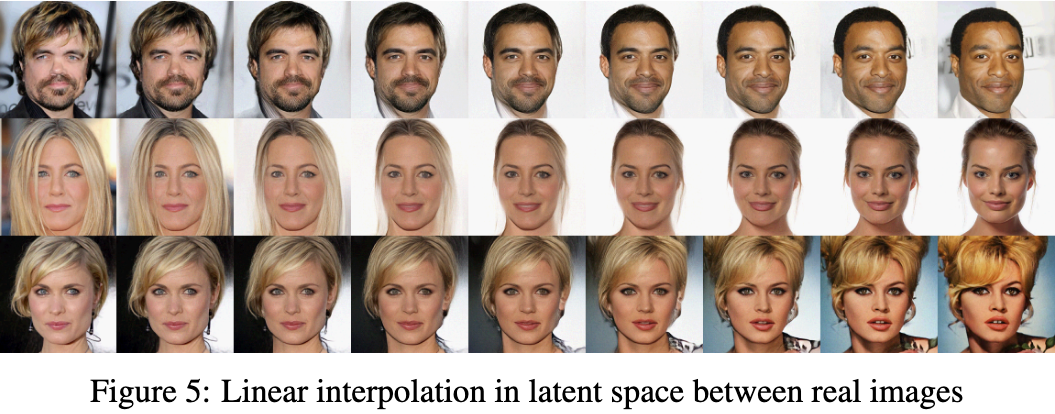
\includegraphics[width=0.75\textwidth]{GLOWInterpolation.png}\\
    \center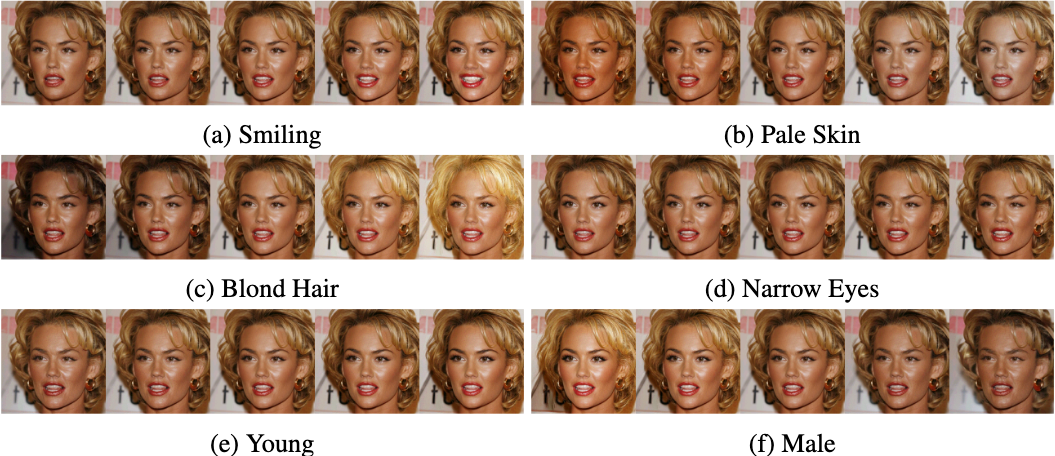
\includegraphics[width=0.75\textwidth]{GLOWLatentSpace.png}\\
\end{frame}

